\section{Algoritmo para el pareamiento de Muones}
Para la identificación de los procesos se implementa un algoritmo para la identificación de los decaimientos a dos muones y la identificacion de los di-muones en él:
\begin{figure}[ht!]
    \centering
    \includegraphics[width=0.84\textwidth]{Analisis_y_Resultados/imagenes/diagrama_pair.png}
    \caption{Diagrama de flujo para la identificación de los pares en los eventos a estudiar.}
    \label{fig:diagrama_pair}
\end{figure}


\section{Caracterizacion de la Señal}

%\begin{figure}[ht!]
%    \centering
    \includegraphics[width=0.84\textwidth]{Analisis_y_Resultados/imagenes/Cambio_de_D0_con_Card.png}
    
    \includegraphics[width=0.84\textwidth]{Analisis_y_Resultados/imagenes/Cambio_de_DZ_con_Card.png}
    
    \includegraphics[width=0.84\textwidth]{Analisis_y_Resultados/imagenes/Cambio_de_Eta_con_Card.png}
    
    \includegraphics[width=0.84\textwidth]{Analisis_y_Resultados/imagenes/Cambio_de_D0_con_Card.png}
    
    \includegraphics[width=0.84\textwidth]{Analisis_y_Resultados/imagenes/Cambio_de_IsolationVar_con_Card.png}
    
    \includegraphics[width=0.84\textwidth]{Analisis_y_Resultados/imagenes/Cambio_de_MassInv_con_Card.png}
    
    
    \includegraphics[width=0.84\textwidth]{Analisis_y_Resultados/imagenes/Cambio_de_Phi_con_Card.png}
    
    
    \includegraphics[width=0.84\textwidth]{Analisis_y_Resultados/imagenes/Cambio_de_PT_con_Card.png}
    
    





%\end{figure}




\begin{figure}[ht!]
    \centering
    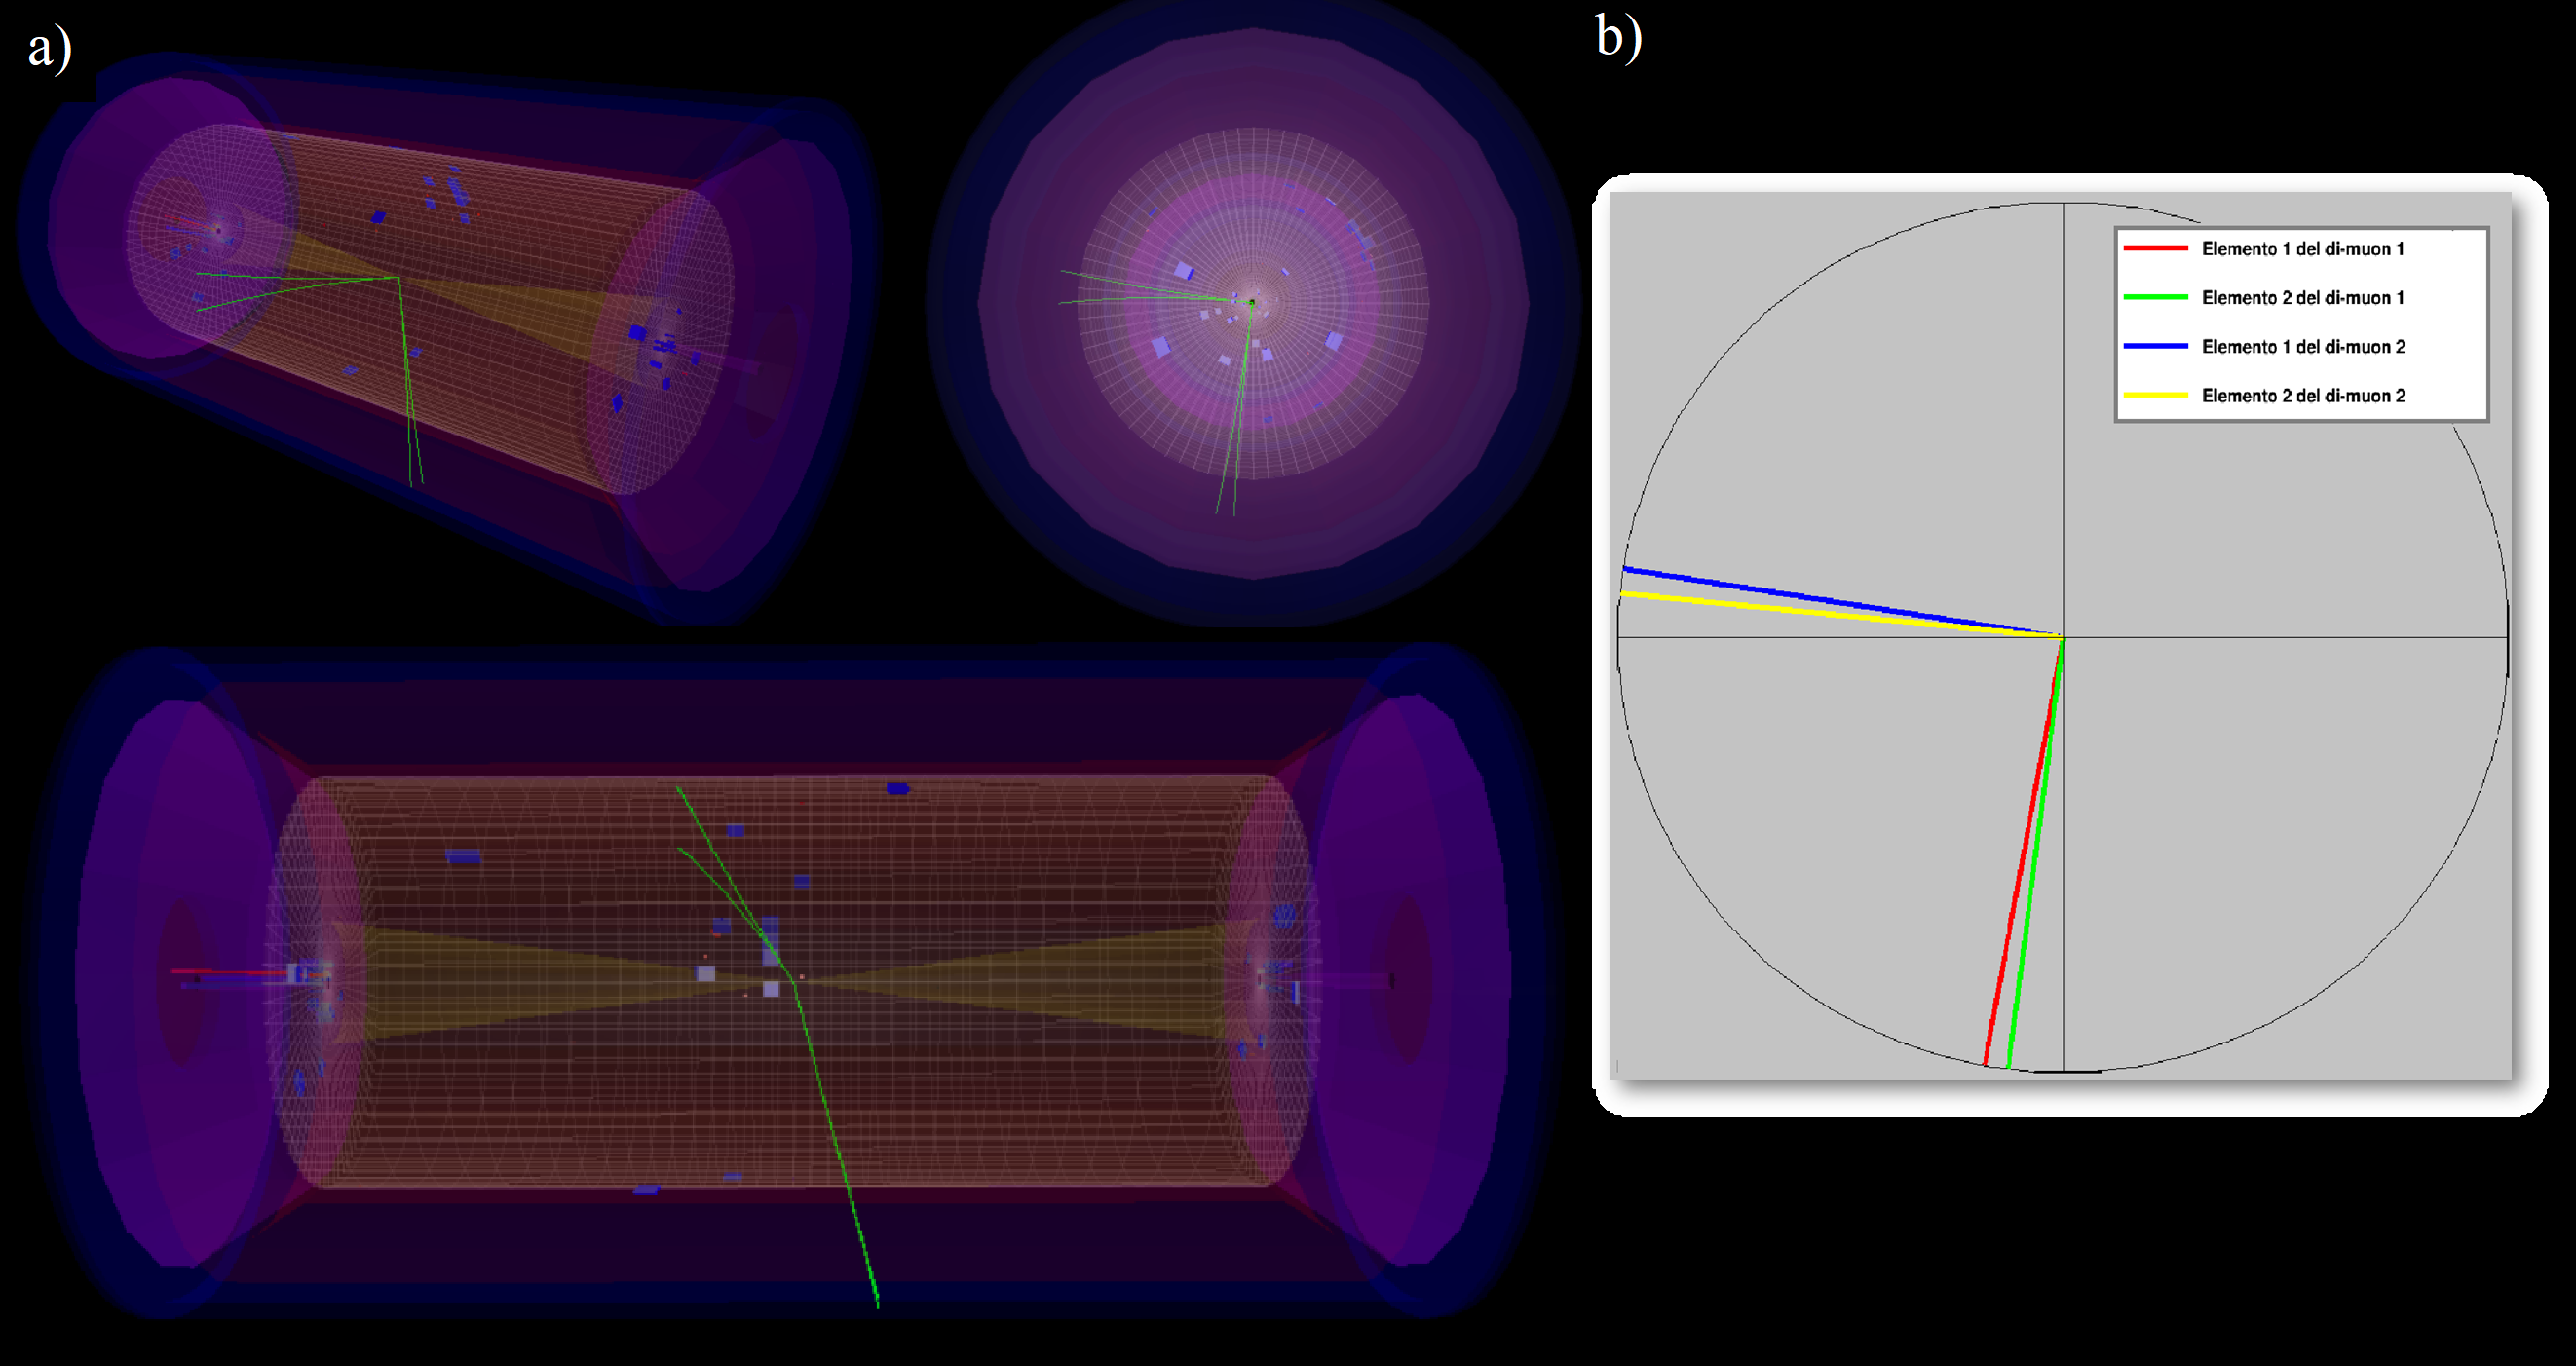
\includegraphics[width=0.84\textwidth]{Analisis_y_Resultados/imagenes/evento_68.png}
    \caption{Representación esquematica de los pares generados en el evento 68 simulado: a) Reconstrucción con EVE; b) Identificación de elementos con C++.}
    \label{fig:diagrama_pair}
\end{figure}
\begin{figure}[ht!]
    \centering
    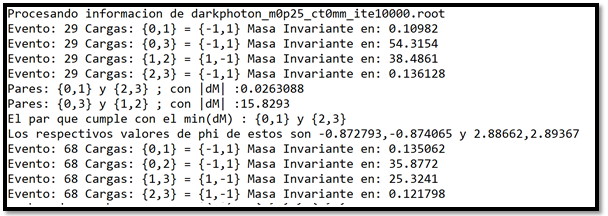
\includegraphics[width=0.84\textwidth]{Analisis_y_Resultados/imagenes/evento_68_info.png}
    \caption{Corte del informe del proceso de selección con C++ del evento 68.}
    \label{fig:diagrama_pair}
\end{figure}
\begin{figure}[ht!]
    \centering
    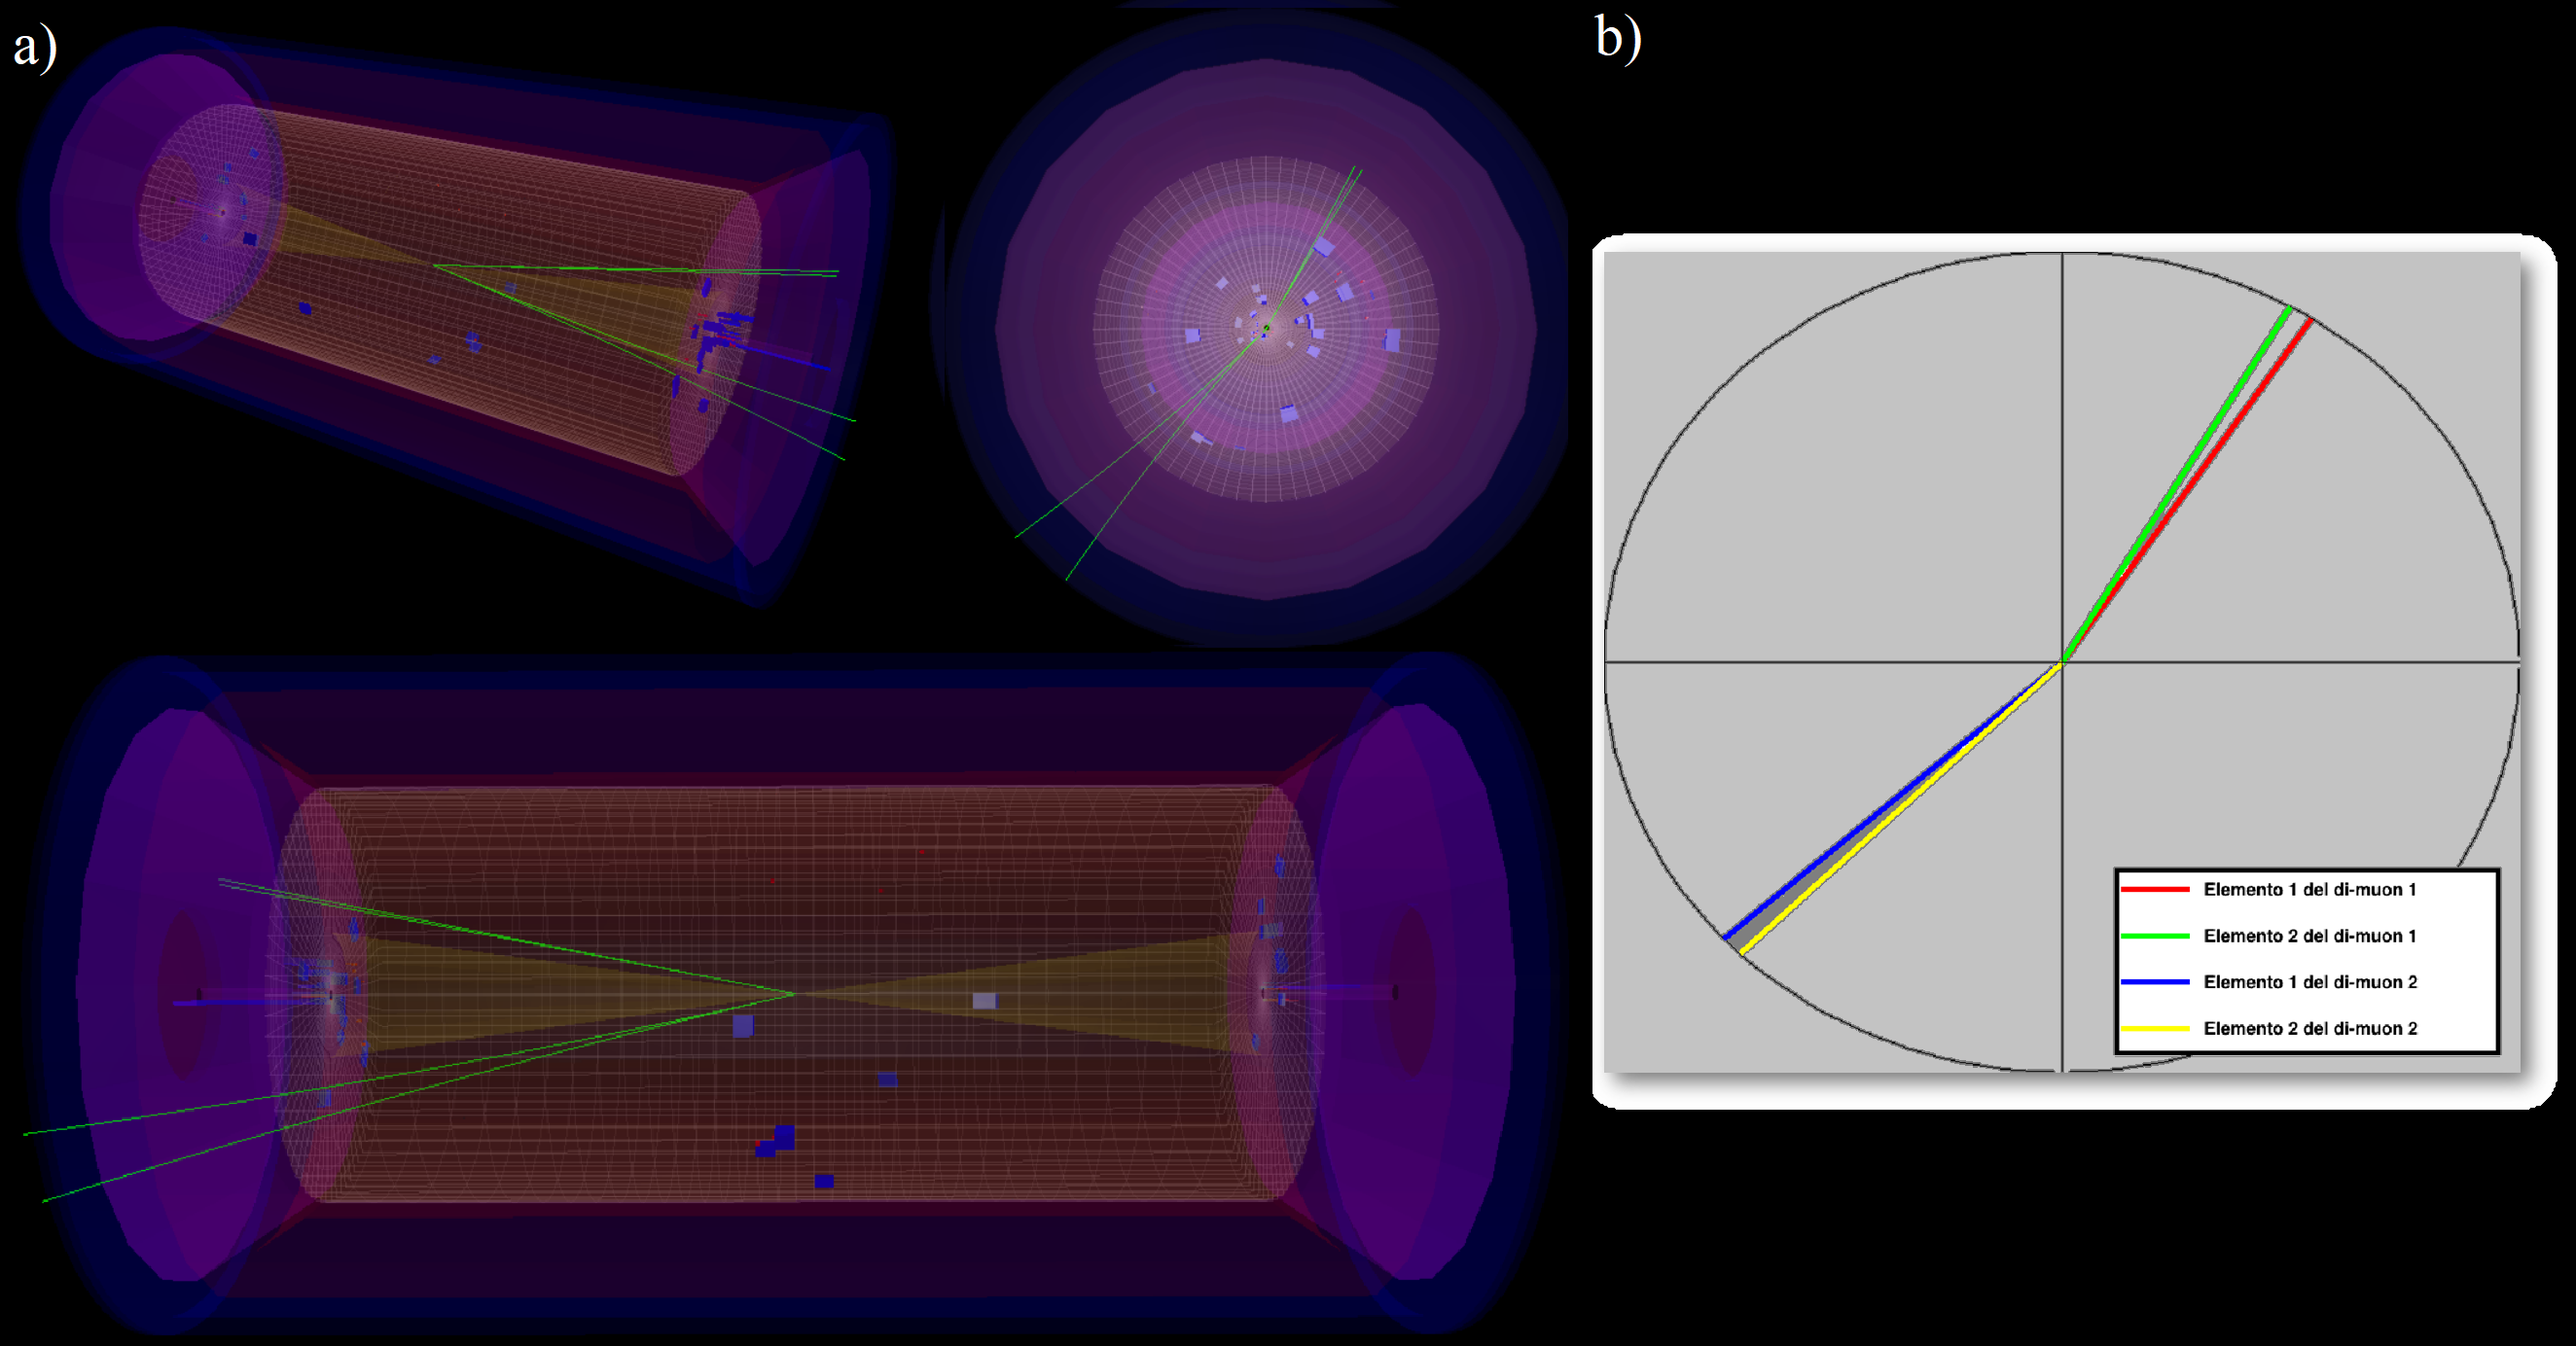
\includegraphics[width=0.84\textwidth]{Analisis_y_Resultados/imagenes/evento_7520.png}
    \caption{Representación esquematica de los pares generados en el evento 7520 simulado: a) Reconstrucción con EVE; b) Identificación de elementos con C++.}
    \label{fig:diagrama_pair}
\end{figure}
\begin{figure}[ht!]
    \centering
    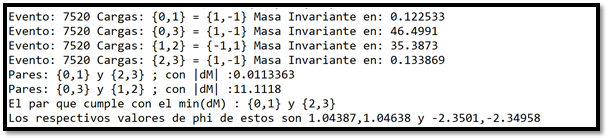
\includegraphics[width=0.84\textwidth]{Analisis_y_Resultados/imagenes/evento_7520_info.png}
    \caption{Corte del informe del proceso de selección con C++ del evento 7520.}
    \label{fig:diagrama_pair}
\end{figure}

\begin{figure}[ht!]
    \centering
    \includegraphics[width=0.84\textwidth]{Analisis_y_Resultados/imagenes/mass.pdf}
    \caption{Masa invariante de los fotones pareados de nuestra se\~nal.}
    \label{fig:diagrama_pair}
\end{figure}

\begin{figure}[ht!]
    \centering
    \includegraphics[width=0.84\textwidth]{Analisis_y_Resultados/imagenes/MASS2.pdf}
    \caption{Masa invariante de los fotones pareados de nuestra se\~nal separados en los menores y los mayores.}
    \label{fig:diagrama_pair}
\end{figure}

\begin{figure}[ht!]
    \centering
    \includegraphics[width=0.84\textwidth]{Analisis_y_Resultados/imagenes/mulPT.pdf}
    \caption{Momento Angular ordenada para cada muon de nuestra se\~nal .}
    \label{fig:diagrama_pair}
\end{figure}



\section{Seleccion de Eventos}

La selecci\'on de eventos considera los cortes a distribuciones necesarios para maximizar la se\~nal y reducir lo mas posible la contribuci\'on 

\begin{table}[]
    \centering
    \begin{tabular}{|c|c|c|c|c|c|}
        \hline\hline
                                        & \multicolumn{5}{|c|}{N\'umero de Eventos HLLHC/CMS} \\

        Selecci\'on                     & c$\tau$=0mm   &  c$\tau$=5mm  & c$\tau$=10mm  & c$\tau$= 50mm & c$\tau$= 100mm\\ \hline
        Total                           & 10,000        & 10,000        & 10,000        & 10,000        & 10,000 \\ \hline
        (muones) $\mu >= 4$               & 1625 / 881    & 902/500       & 433/227       & 39/16         & 6/2 \\ \hline
        (di-muones)$\mu^+ \mu^->~= ~ 2$ & 1625 / 881    & 902/500       & 433/227       & 39/16         & 6/2 \\ \hline
        Isolation $<~ 2 GeV$            &               &               &               &               & \\ \hline\hline
    \end{tabular}
    \caption{Selecci\'on de eventos para muestras con masa de ``dark photon'' de $\gamma_{D}^{m}$ = 0.25 GeV}
    \label{tab:my_label}
\end{table}